\documentclass[14pt,aspectratio=169]{beamer}
\usepackage{polyglossia}
\setdefaultlanguage{english}
\usetheme{SaintPetersburg}

\usepackage{amsthm}
\usepackage{amssymb}
\usepackage{amsmath}
\usepackage{mathtools}
\usepackage{listings}
\usepackage{booktabs}
\usepackage{graphicx}
\usepackage{tikz}

\graphicspath{{figures/}}

\newcommand{\Fourier}[1]{\mathcal{F}\left\{#1\right\}}
\newcommand{\InverseFourier}[1]{\mathcal{F}^{-1}\left\{#1\right\}}
\newcommand{\Var}[1]{\sigma_{#1}^2}

\AtBeginSection[]{
%	\iffirstsection
%		\begin{frame}{Plan}
%			\tableofcontents
%		\end{frame}
%		\firstsectionfalse
%	\fi
%	\begin{frame}{Plan}
%		\tableofcontents[currentsection]
%	\end{frame}
	\frame{\sectionpage}
}

\title{Generating standing and propagating ocean waves with three-dimensional ARMA model}
\subtitle{Technical report}
\author{Ivan Gankevich}
\date{Aug 26, 2016}

\begin{document}

	\frame{\maketitle}

	\section{Two methods of finding wave's ACF}

	\begin{frame}
		\frametitle{Analytic method}
		\only<1>{%
			Apply Wiener---Khinchin theorem to a wave profile $\zeta$ to get ACF $K$:
			\begin{equation*}
				K(t) = \Fourier{\left| \zeta(t) \right|^2}.
				\label{eq:wiener-khinchin}
			\end{equation*}%
		}
		\only<2>{%
			\begin{example}
				Standing wave profile:
				\begin{equation*}
					\zeta(t, x, y) = A \sin (k_x x + k_y y) \sin (\sigma t).
					\label{eq:standing-wave}
				\end{equation*}
				Standing wave ACF:
				\begin{equation*}
					K(t,x,y) =
					\gamma
					\exp\left[-\alpha (|t|+|x|+|y|) \right]
					\cos \beta t
					\cos \left[ \beta x + \beta y \right].
					\label{eq:standing-wave-acf}
				\end{equation*}
			\end{example}%
		}
		\only<3>{%
			\begin{example}
				Propagating wave profile:
				\begin{equation*}
					\zeta(t, x, y) = A \cos (\sigma t + k_x x + k_y y).
					\label{eq:propagating-wave}
				\end{equation*}
				Propagating wave ACF:
				\begin{equation*}
					K(t,x,y) =
					\gamma
					\exp\left[-\alpha (|t|+|x|+|y|) \right]
					\cos\left[\beta (t+x+y) \right].
					\label{eq:propagating-wave-acf}
				\end{equation*}
			\end{example}%
		}
		\only<4>{%
			Some observations:
			\begin{itemize}
				\item Taking Fourier transform of sine/cosine wave profile requires
					  multiplying it by an decaying exponent to produce useful ACF.
				\item Fourier Transform of squared exponent (Gaussian) is another Gaussian.
			\end{itemize}
			\vfill\centering%
			\alert{Why use Fourier transform at all?}%
		}
	\end{frame}

	\begin{frame}
		\frametitle{Empirical method}
		The algorithm:
		\begin{enumerate}
			\item Multiply wave profile by an decaying exponent.
			\item Adjust sine/cosine phase to move maximum value to the origin
				  (or substitute sine with cosine to get the same effect).
		\end{enumerate}
		\vfill%
		In case of plain waves result is the same as for analitic method.
	\end{frame}

	\section{Governing equations for 3-dimensional ARMA process}

	\begin{frame}
		\frametitle{3-D ARMA process}
		Three-dimensional autoregressive moving average process is defined by
		\begin{equation*}
			\zeta_{i,j,k} =
			\sum\limits_{l=0}^{p_1}
			\sum\limits_{m=0}^{p_2}
			\sum\limits_{n=0}^{p_3}
			\Phi_{l,m,n} \zeta_{i-l,j-m,k-n}
			+
			\sum\limits_{l=0}^{q_1}
			\sum\limits_{m=0}^{q_2}
			\sum\limits_{n=0}^{q_3}
			\Theta_{l,m,n} \epsilon_{i-l,j-m,k-n}
			,
			\label{eq:arma-process}
		\end{equation*}
		\small{%
			where $\zeta$ --- wave elevation, $\Phi$ --- AR coefficients, $\Theta$ --- MA
			coefficients, \newline$\epsilon$ --- white noise with Gaussian distribution,
			$(p_1,p_2,p_3)$ --- AR process order, $(q_1,q_2,q_3)$ --- MA process order, and
			$\Phi_{0,0,0} \equiv 0$, $\Theta_{0,0,0} \equiv 0$.% 
		}
	\end{frame}

	\begin{frame}
		\frametitle{Determining coefficients}
		\framesubtitle{AR process}
		\small%
		Solve linear system of equations (3-D Yule---Walker equations) for $\Phi$:
		\begin{equation*}
		    \Gamma
		    \left[
		        \begin{array}{l}
		            \Phi_{0,0,0}\\
		            \Phi_{0,0,1}\\
		            \vdotswithin{\Phi_{0,0,0}}\\
		            \Phi_{p_1,p_2,p_3}
		        \end{array}
		    \right]
		    = 
		    \left[
		        \begin{array}{l}
		            K_{0,0,0}-\Var{\epsilon}\\
		            K_{0,0,1}\\
		            \vdotswithin{K_{0,0,0}}\\
		            K_{p_1,p_2,p_3}
		        \end{array}
		    \right],
		    \qquad
		    \Gamma=
		    \left[
		        \begin{array}{llll}
		            \Gamma_0 & \Gamma_1 & \cdots & \Gamma_{p_1} \\
		            \Gamma_1 & \Gamma_0 & \ddots & \vdotswithin{\Gamma_0} \\
		            \vdotswithin{\Gamma_0} & \ddots & \ddots & \Gamma_1 \\
		            \Gamma_{p_1} & \cdots & \Gamma_1 & \Gamma_0
		        \end{array}
		    \right],
		\end{equation*}
		\begin{equation*}
			\Gamma_i = 
			\left[
			\begin{array}{llll}
				\Gamma^0_i & \Gamma^1_i & \cdots & \Gamma^{p_2}_i \\
				\Gamma^1_i & \Gamma^0_i & \ddots & \vdotswithin{\Gamma^0_i} \\
				\vdotswithin{\Gamma^0_i} & \ddots & \ddots & \Gamma^1_i \\
				\Gamma^{p_2}_i & \cdots & \Gamma^1_i & \Gamma^0_i
			\end{array}
			\right]
			\qquad
			\Gamma_i^j= 
			\left[
			\begin{array}{llll}
				K_{i,j,0} & K_{i,j,1} & \cdots & K_{i,j,p_3} \\
				K_{i,j,1} & K_{i,j,0} & \ddots &x \vdotswithin{K_{i,j,0}} \\
				\vdotswithin{K_{i,j,0}} & \ddots & \ddots & K_{i,j,1} \\
				K_{i,j,p_3} & \cdots & K_{i,j,1} & K_{i,j,0}
			\end{array}
			\right].
		\end{equation*}
	\end{frame}

	\begin{frame}
		\frametitle{Determining coefficients}
		\framesubtitle{MA process}
		\small%
		Solve non-linear system of equations for $\Theta$:
		\begin{equation*}
			K_{i,j,k} = 
			\left[
				\displaystyle
				\sum\limits_{l=i}^{q_1}
				\sum\limits_{m=j}^{q_2}
				\sum\limits_{n=k}^{q_3}
				\Theta_{l,m,n}\Theta_{l-i,m-j,n-k}
			\right]
			\Var{\epsilon}
		\end{equation*}
		via fixed-point iteration method:
		\begin{equation*}
			\theta_{i,j,k} =
				-\frac{K_{0,0,0}}{\Var{\epsilon}}
				+
				\sum\limits_{l=i}^{q_1}
				\sum\limits_{m=j}^{q_2}
				\sum\limits_{n=k}^{q_3}
				\Theta_{l,m,n} \Theta_{l-i,m-j,n-k}.
		\end{equation*}
	\end{frame}

	\begin{frame}
		\frametitle{Determining coefficients}
		\framesubtitle{ARMA process}
		To mix processes one needs to divide ACF between processes, and
		recompute one of the parts to match process properties (mean,
		variance etc.).
		\vfill%
		\begin{center}
			\alert{There is no recomputation formula for 3-D proccess.}
		\end{center}
	\end{frame}

	\begin{frame}
		\frametitle{Our approach}
		Use AR process for standing waves and MA process for
		propagating waves.
		\vfill%
		Supporting experimental results:
		\begin{itemize}
			\item It works that way in practice.
			\item It does not work the other way round
				  (processes diverge).
			\item Wavy surface integral characteristics 
				  match the ones of real ocean waves.
		\end{itemize}
	\end{frame}

	\section{Evaluation and verification}

	\begin{frame}
		\frametitle{Experiment setup}
		\begin{itemize}
			\item Generate standing/propagating waves with
				  AR/MA processes respectively.
			\item Estimate distributions of integral
				  characteristics.
			\item Compare estimated distributions to the
				  known ones via QQ plots.
		\end{itemize}
		\vfill%
		\begin{center}
			\small
			\begin{tabular}{ll}
				\toprule
				Characteristic & Weibull shape ($k$) \\
				\midrule
				Wave height & 2 \\
				Wave length & 2.3 \\
				Crest length & 2.3 \\
				Wave period & 3 \\
				Wave slope & 2.5 \\
				Three-dimensionality & 2.5 \\
				\bottomrule
			\end{tabular}%
		\end{center}
	\end{frame}

%	\begin{frame}
%		\frametitle{Input ACFs (time slices)}
%		Standing wave ACF:
%		\vfill%
%		\begin{tabular}{llll}%
%			\includegraphics[scale=0.45]{standing-acf-0} &
%			\includegraphics[scale=0.45]{standing-acf-1} &
%			\includegraphics[scale=0.45]{standing-acf-3} &
%			\includegraphics[scale=0.45]{standing-acf-4} \\
%		\end{tabular}
%		\vfill%
%		Propagating wave ACF:
%		\vfill%
%		\begin{tabular}{llll}%
%			\includegraphics[scale=0.45]{propagating-acf-00} &
%			\includegraphics[scale=0.45]{propagating-acf-01} &
%			\includegraphics[scale=0.45]{propagating-acf-03} &
%			\includegraphics[scale=0.45]{propagating-acf-04} \\
%		\end{tabular}
%	\end{frame}

	\begin{frame}
		\frametitle{Verification results (QQ plots)}
		\small%
		\centering
		\begin{columns}
			\begin{column}{0.5\textwidth}
				\centering%
				Standing waves
				\begin{tabular}{ll}
					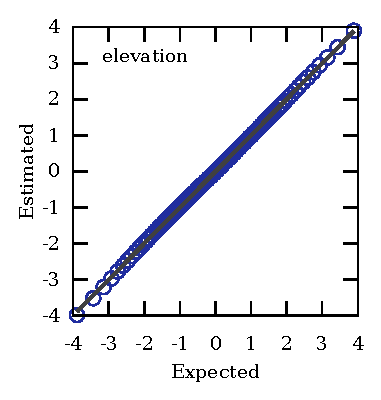
\includegraphics[scale=0.5]{standing-elevation} &
					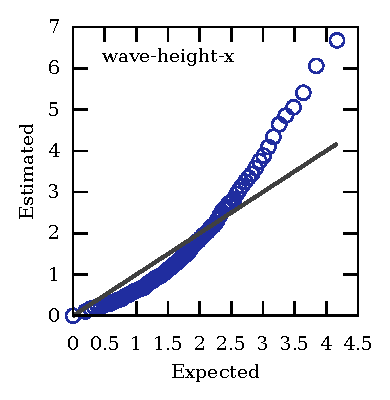
\includegraphics[scale=0.5]{standing-wave-height-x} \\
					\addlinespace
					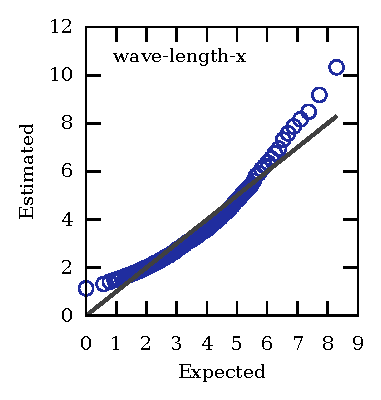
\includegraphics[scale=0.5]{standing-wave-length-x} &
					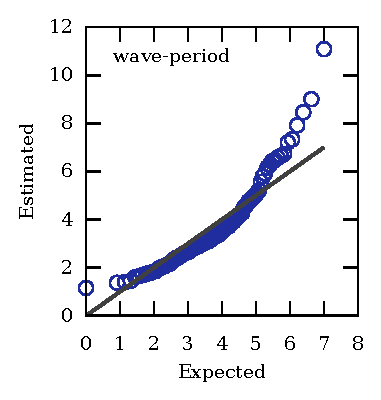
\includegraphics[scale=0.5]{standing-wave-period} \\
				\end{tabular}
			\end{column}
			\begin{column}{0.5\textwidth}
				\centering%
				Propagating waves
				\begin{tabular}{ll}
					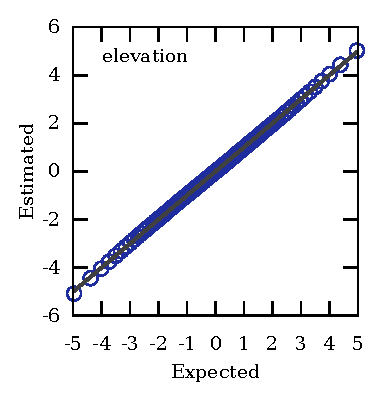
\includegraphics[scale=0.5]{propagating-elevation} &
					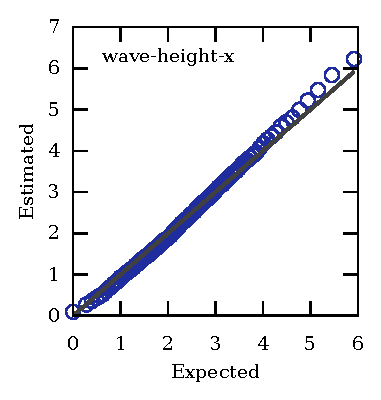
\includegraphics[scale=0.5]{propagating-wave-height-x} \\
					\addlinespace
					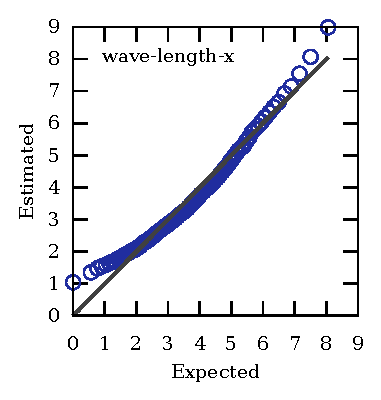
\includegraphics[scale=0.5]{propagating-wave-length-x} &
					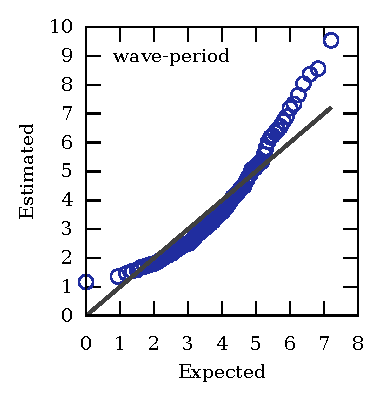
\includegraphics[scale=0.5]{propagating-wave-period} \\
				\end{tabular}
			\end{column}
		\end{columns}
	\end{frame}

\end{document}
